\chapter{準備}
\label{ch:seminar-00}

\begin{definition}{有限集合と濃度（finite set, cardinality）}{sem-finite}
  集合 $S$ が\textbf{有限集合}であるとは，ある $n \in \N$ と
  全単射 $f \colon \range{n} \to S$ が存在することをいう．
  この $n$ を $S$ の\textbf{濃度}といい $|S|$ で表す．
\end{definition}

\begin{claim}{有限集合の最小元}{sem-finite-min}
  $\R$ の空でない有限部分集合 $S$（定義~\ref{def:sem-finite}）には
  最小元が存在する：
  \[
    \exists\, s^* \in S \;\;\text{s.t.}\;\; \forall\, s \in S,\; s^* \leq s.
  \]
\end{claim}

\begin{proof}
  $|S|$ に関する帰納法で示す．

  \textbf{$|S| = 1$ の時．} $S$ の唯一の元がそのまま最小元．

  \textbf{$|S| \geq 2$ の時．}
  $\R$ の任意の空でない有限部分集合 $T$ について $|T| < |S|$ ならば最小元を持つと仮定する．
  $a \in S$ を任意に取り $S' \defeq S \setminus \{a\}$ とおくと $|S'| = |S| - 1$ なので，
  仮定が $S'$ に対して適用でき最小元 $b \in S'$ を持つ．
  $a, b \in \R$ より $b \leq a$ か $a < b$ のいずれかが成り立つので，
  \[
    s^* \defeq
    \begin{cases}
      b & (b \leq a), \\
      a & (a < b)
    \end{cases}
  \]
  とおけば $s^* \in S$ かつ任意の $s \in S$ について $s^* \leq s$．
\end{proof}

%% ============================================================
%% 線形代数
%% ============================================================
\section{線形代数}
\label{sec:sem-linalg}

\subsection{置換}
\label{sec:sem-permutation}

\begin{definition}{置換（permutation）}{sem-permutation}
  $n \in \N$ とする．$\range{n}$ 上の\textbf{置換}全体の集合を
  \[
    \Perm(n) \defeq \{\sigma \colon \range{n} \to \range{n} \mid \sigma \text{ は全単射}\}
  \]
  と定める．$|\Perm(n)| = n!$ である．
\end{definition}

\subsection{フロベニウス内積}
\label{sec:sem-frobenius-inner}

\begin{definition}{フロベニウス内積（Frobenius inner product）}{sem-frobenius-inner}
  同じサイズの2つの行列 $\mathbf{A}, \mathbf{B} \in \R^{n \times m}$ に対し，
  \textbf{フロベニウス内積}を
  \[
    \inner{\mathbf{A}}{\mathbf{B}}
    \defeq \tr(\mathbf{A}^\top \mathbf{B})
    = \sum_{i=1}^{n} \sum_{j=1}^{m} A_{i,j} B_{i,j}
  \]
  で定める．
\end{definition}

%% ============================================================
%% 距離空間
%% ============================================================
\section{距離空間}
\label{sec:sem-metric-space}

\begin{definition}{距離空間（metric space）}{sem-metric-space}
  集合 $\Omega$ と関数 $d \colon \Omega \times \Omega \to [0, \infty)$ の組
  $(\Omega, d)$ が\textbf{距離空間}であるとは，
  次の3条件がすべての $x, y, z \in \Omega$ に対して成り立つことをいう：
  \begin{enumerate}
    \item[(i)] 同一性：$d(x, y) = 0 \iff x = y$，
    \item[(ii)] 対称性：$d(x, y) = d(y, x)$，
    \item[(iii)] 三角不等式：$d(x, z) \leq d(x, y) + d(y, z)$．
  \end{enumerate}
  関数 $d$ を $\Omega$ 上の\textbf{距離関数}という．
\end{definition}

\begin{definition}{開球・開集合・距離位相}{sem-metric-topology}
  距離空間 $(\Omega, d)$ 上の点 $x \in \Omega$ と半径 $r > 0$ に対して，
  \textbf{開球}を
  \[
    B_r(x) \defeq \{y \in \Omega \mid d(x, y) < r\}
  \]
  で定める．
  部分集合 $U \subset \Omega$ が\textbf{開集合}であるとは，
  任意の $x \in U$ に対してある $r > 0$ が存在して
  $B_r(x) \subset U$ となることをいう．
  $\Omega$ の開集合全体を $(\Omega, d)$ の\textbf{距離位相}と呼ぶ．
\end{definition}

\begin{definition}{完備距離空間（complete metric space）}{sem-complete-metric}
  距離空間 $(\Omega, d)$ の列 $(x_n)_{n \geq 1}$ が\textbf{Cauchy 列}であるとは，
  任意の $\varepsilon > 0$ に対してある $N \in \N$ が存在して
  $n, m \geq N \Longrightarrow d(x_n, x_m) < \varepsilon$ となることをいう．
  $(\Omega, d)$ が\textbf{完備}であるとは，
  $\Omega$ 上のすべての Cauchy 列が $\Omega$ の点に収束することをいう．
\end{definition}

\begin{definition}{可分距離空間（separable metric space）}{sem-separable}
  距離空間 $(\Omega, d)$ の部分集合 $D \subset \Omega$ が\textbf{稠密}であるとは，
  任意の $x \in \Omega$ と任意の $\varepsilon > 0$
  に対して $d(x, y) < \varepsilon$ を満たす $y \in D$ が存在することをいう．
  $\Omega$ が可算な稠密部分集合を持つとき，$\Omega$ は\textbf{可分}であるという．
\end{definition}

\begin{definition}{Hausdorff 性（Hausdorff property）}{sem-hausdorff}
  距離空間 $(\Omega, d)$ が\textbf{Hausdorff 空間}であるとは，
  相異なる任意の 2 点 $x, y \in \Omega$ に対し，
  $B_r(x) \cap B_r(y) = \emptyset$ をみたす $r > 0$ が存在することをいう．
\end{definition}

\begin{claim}{距離空間は Hausdorff}{sem-metric-hausdorff}
  任意の距離空間は Hausdorff である．
  特に単点集合 $\{x\}$ および有限集合 $\{x_1, \ldots, x_n\}$ は閉集合．
\end{claim}

\begin{proof}
  相異なる $x, y \in \Omega$ に対し $r \defeq d(x, y)/2 > 0$ とおく．
  $z \in B_r(x) \cap B_r(y)$ ならば三角不等式より
  $d(x, y) \leq d(x, z) + d(z, y) < 2r = d(x, y)$ となり矛盾．
  ゆえに $B_r(x) \cap B_r(y) = \emptyset$．

  単点 $\{x\}$ の閉性：任意の $y \neq x$ に対し
  $r' \defeq d(x, y)/2 > 0$ で $B_{r'}(y) \cap \{x\} = \emptyset$
  ゆえ $\Omega \setminus \{x\}$ は開集合，すなわち $\{x\}$ は閉集合．
  有限集合は閉集合の有限和ゆえ閉．
\end{proof}

\begin{definition}{第二可算（second-countable）}{sem-second-countable}
  距離空間 $(\Omega, d)$ が\textbf{第二可算}であるとは，
  可算な開集合族 $\mathcal{N} = \{U_k\}_{k \geq 1}$ が存在して，
  $\Omega$ の任意の開集合 $U$ がある部分族 $\mathcal{N}' \subset \mathcal{N}$ の和集合
  $U = \bigcup_{V \in \mathcal{N}'} V$ として書けることをいう．
  この $\mathcal{N}$ を\textbf{可算開基（countable base）}という．
\end{definition}

\begin{definition}{Lindelöf 性（Lindel\"of property）}{sem-lindelof}
  距離空間 $(\Omega, d)$ が\textbf{Lindelöf 空間}であるとは，
  $\Omega$ の任意の開部分集合 $U$ の任意の開被覆 $\{V_\lambda\}_{\lambda \in \Lambda}$
  （$U \subset \bigcup_\lambda V_\lambda$）が可算な部分被覆を持つことをいう．
\end{definition}

\begin{claim}{可分距離空間は第二可算かつ Lindelöf}{sem-separable-second-countable-lindelof}
  可分距離空間 $(\Omega, d)$ は第二可算であり，かつ Lindelöf である．
\end{claim}

\begin{proof}
  \textbf{第二可算性．}
  $D = \{q_k\}_{k \geq 1} \subset \Omega$ を可算稠密部分集合とし，
  $\mathcal{N} \defeq \{B_{1/n}(q_k) \mid k \geq 1,\, n \geq 1\}$ とおく．
  $\mathcal{N}$ は可算族．任意の開集合 $U$ と $x \in U$ に対し
  $B_r(x) \subset U$ をみたす $r > 0$ がとれる．
  $2/n < r$ なる $n \in \N$ と，稠密性から $d(q_k, x) < 1/n$ なる $q_k \in D$ をとると，
  $x \in B_{1/n}(q_k)$ かつ，$z \in B_{1/n}(q_k)$ について
  $d(z, x) \leq d(z, q_k) + d(q_k, x) < 2/n < r$ ゆえ
  $B_{1/n}(q_k) \subset B_r(x) \subset U$．
  したがって $U$ は $\mathcal{N}$ の部分族の和集合として書ける．

  \textbf{Lindelöf 性．}
  $\mathcal{N} = \{U_k\}_{k \geq 1}$ を可算開基，$U$ を開集合，
  $\{V_\lambda\}_{\lambda \in \Lambda}$ を $U$ の開被覆とする．
  各 $x \in U$ に対し $x \in V_{\lambda(x)}$ なる $\lambda(x)$ をひとつ選ぶと，
  $V_{\lambda(x)}$ は開ゆえある $k(x) \geq 1$ で $x \in U_{k(x)} \subset V_{\lambda(x)}$．
  $K \defeq \{k(x) \mid x \in U\} \subset \N$ は可算．
  各 $k \in K$ に対し $U_k \subset V_{\lambda_k}$ なる $\lambda_k \in \Lambda$ をひとつ選ぶと，
  $\bigcup_{k \in K} V_{\lambda_k} \supset \bigcup_{k \in K} U_k \supset U$
  ゆえ $\{V_{\lambda_k}\}_{k \in K}$ は可算部分被覆．
\end{proof}

\begin{definition}{Polish 空間（Polish space）}{sem-polish}
  完備かつ可分な距離空間を\textbf{Polish 空間}という．
  例：$\R^d$ はユークリッド距離に関して Polish 空間である
  （$\Q^d$ が可算稠密部分集合を与える）．
\end{definition}

%% ============================================================
%% 測度論
%% ============================================================
\section{測度論}
\label{sec:sem-measure-theory}

\subsection{可測空間と確率測度}
\label{sec:sem-measurable}

\begin{definition}{$\sigma$-代数（$\sigma$-algebra）}{sem-sigma-algebra}
  集合 $\Omega$ の部分集合族 $\mathcal{F} \subset 2^{\Omega}$ が
  \textbf{$\sigma$-代数}であるとは，
  以下の3条件を満たすことをいう：
  \begin{enumerate}
    \item[(i)] $\Omega \in \mathcal{F}$，
    \item[(ii)] $A \in \mathcal{F} \Longrightarrow A^c \in \mathcal{F}$（補集合で閉じる），
    \item[(iii)] $A_1, A_2, \ldots \in \mathcal{F} \Longrightarrow
      \bigcup_{k=1}^{\infty} A_k \in \mathcal{F}$（可算合併で閉じる）．
  \end{enumerate}
\end{definition}

\begin{definition}{可測空間（measurable space）}{sem-measurable-space}
  集合 $\Omega$ と $\Omega$ 上の $\sigma$-代数 $\mathcal{F}$ の組
  $(\Omega, \mathcal{F})$ を\textbf{可測空間}という．
  $\mathcal{F}$ の元を\textbf{可測集合}という．
\end{definition}

\begin{definition}{可測写像}{sem-measurable-map}
  可測空間 $(\Omega_1, \mathcal{F}_1)$ から $(\Omega_2, \mathcal{F}_2)$ への
  写像 $T \colon \Omega_1 \to \Omega_2$ が\textbf{可測}であるとは，
  $T^{-1}(A) \in \mathcal{F}_1$ がすべての $A \in \mathcal{F}_2$ に対して成り立つことをいう．
\end{definition}

\begin{definition}{ボレル $\sigma$-代数}{sem-borel}
  距離空間 $(\Omega, d)$ のすべての開集合（定義~\ref{def:sem-metric-topology}）
  を含む最小の $\sigma$-代数を
  \textbf{ボレル $\sigma$-代数}といい，$\Bb(\Omega)$ と記す．
\end{definition}

\begin{definition}{可測関数（measurable function）}{sem-measurable-function}
  可測空間 $(\Omega, \mathcal{F})$ から $(\R, \Bb(\R))$ への可測写像
  $f \colon \Omega \to \R$（定義~\ref{def:sem-measurable-map}）を
  \textbf{可測関数}という．
  特に Polish 空間 $\X$ にボレル $\sigma$-代数 $\Bb(\X)$ を入れた
  可測空間上の可測関数を\textbf{ボレル可測関数}ともいう．
\end{definition}

\begin{definition}{積可測空間（product measurable space）}{sem-product-measurable}
  距離空間 $(\X, d_\X)$, $(\Y, d_\Y)$ に対して，
  積空間 $\X \times \Y$ に\textbf{積距離}
  \[
    d\bigl((x, y), (x', y')\bigr) \defeq d_\X(x, x') + d_\Y(y, y')
  \]
  を入れたときのボレル $\sigma$-代数を $\Bb(\X \times \Y)$ と記し，
  可測空間 $(\X \times \Y, \Bb(\X \times \Y))$ を
  $(\X, \Bb(\X))$ と $(\Y, \Bb(\Y))$ の\textbf{積可測空間}という．
\end{definition}

\begin{definition}{測度（measure）}{sem-measure}
  可測空間 $(\Omega, \mathcal{F})$ 上の\textbf{測度}とは，
  関数 $\mu \colon \mathcal{F} \to [0, \infty]$ であって，
  次の 2 条件を満たすものをいう：
  \begin{enumerate}
    \item[(i)] $\mu(\emptyset) = 0$，
    \item[(ii)] 互いに素な可測集合 $A_1, A_2, \ldots \in \mathcal{F}$ に対して
      $\mu\bigl(\bigcup_{k=1}^{\infty} A_k\bigr) = \sum_{k=1}^{\infty} \mu(A_k)$
      （可算加法性）．
  \end{enumerate}
\end{definition}

\begin{definition}{確率測度（probability measure）}{sem-probability-measure}
  可測空間 $(\Omega, \mathcal{F})$ 上の測度 $\mu$ が $\mu(\Omega) = 1$ を満たすとき，
  $\mu$ を\textbf{確率測度}という．
  $\Omega$ 上の確率測度の全体を $\Mm_+^1(\Omega)$ と記す．
\end{definition}

\subsection{測度に対する積分}
\label{sec:sem-integration}

\begin{definition}{指示関数（indicator function）}{sem-indicator}
  集合 $\Omega$ の部分集合 $A \subset \Omega$ に対して，
  \textbf{指示関数} $\mathbf{1}_A \colon \Omega \to \{0, 1\}$ を
  \[
    \mathbf{1}_A(y) \defeq
    \begin{cases}
      1 & y \in A, \\
      0 & y \notin A
    \end{cases}
  \]
  で定める．
\end{definition}

\begin{definition}{単関数（simple function）}{sem-simple-function}
  可測空間 $(\Omega, \mathcal{F})$ 上の関数 $s \colon \Omega \to \R_+$ が
  \textbf{単関数}であるとは，互いに素な可測集合
  $A_1, \ldots, A_m \in \mathcal{F}$ と非負定数 $c_1, \ldots, c_m \geq 0$ を用いて
  \[
    s = \sum_{k=1}^{m} c_k \mathbf{1}_{A_k}
  \]
  と表せることをいう．
\end{definition}

\begin{definition}{非負可測関数の積分}{sem-nonneg-integral}
  可測空間 $(\Omega, \mathcal{F})$ 上の測度 $\mu$ に対し，
  非負可測関数の積分を以下の 2 段階で定める：
  \begin{itemize}
    \item[(i)] 単関数 $s = \sum_{k=1}^{m} c_k \mathbf{1}_{A_k}$
      （定義~\ref{def:sem-simple-function}）の積分を
      \[
        \int_\Omega s \, \d\mu \defeq \sum_{k=1}^{m} c_k \, \mu(A_k)
      \]
      で定める．
    \item[(ii)] 非負可測関数 $f \colon \Omega \to [0, \infty]$ の積分を
      \[
        \int_\Omega f \, \d\mu \defeq
        \sup\!\left\{ \int_\Omega s \, \d\mu
        \;\middle|\; s \text{ は単関数}, \; 0 \leq s \leq f \right\}
      \]
      で定める．この値は常に $[0, +\infty]$ に存在し well-defined である．
  \end{itemize}
\end{definition}

\begin{proposition}{単調収束定理と単関数近似（monotone convergence theorem, MCT）}{sem-mct}
  可測空間 $(\Omega, \mathcal{F})$ 上の測度 $\mu$ に対して次が成り立つ．
  \begin{enumerate}
    \item[(i)] \textbf{単関数近似}：任意の非負可測関数
      $f \colon \Omega \to [0, \infty]$ に対して，
      各点で $f_n \uparrow f$ を満たす単関数の単調増加列 $(f_n)_{n \geq 1}$ が存在する．
    \item[(ii)] \textbf{単調収束定理}：
      非負可測関数の単調増加列 $f_n \uparrow f$ に対して
      $\int f_n \, \d\mu \uparrow \int f \, \d\mu$．
  \end{enumerate}
\end{proposition}

\begin{proposition}{積分の測度に関する線形性}{sem-measure-linearity}
  可測空間 $(\Omega, \mathcal{F})$ 上の測度 $\mu_1, \ldots, \mu_n$，
  非負係数 $a_1, \ldots, a_n \geq 0$，および非負可測関数
  $f \colon \Omega \to [0, \infty]$ に対して，
  \[
    \int_\Omega f \, \d\!\Bigl(\sum_{i=1}^{n} a_i \mu_i\Bigr)
    = \sum_{i=1}^{n} a_i \int_\Omega f \, \d\mu_i.
  \]
  ここで測度の和・スカラー倍は可測集合 $A \in \mathcal{F}$ に対して
  $(\mu_1 + \mu_2)(A) \defeq \mu_1(A) + \mu_2(A)$，
  $(a\mu)(A) \defeq a\, \mu(A)$ で定まる測度である．
\end{proposition}

\begin{proof}
  単関数 $s = \sum_{k} c_k \mathbf{1}_{A_k}$ について，
  単関数積分の定義と測度の和・スカラー倍の定義から
  \[
    \int s \, \d\!\Bigl(\sum_i a_i \mu_i\Bigr)
    = \sum_k c_k \Bigl(\sum_i a_i \mu_i\Bigr)(A_k)
    = \sum_k c_k \sum_i a_i \mu_i(A_k)
    = \sum_i a_i \sum_k c_k \mu_i(A_k)
    = \sum_i a_i \int s \, \d\mu_i.
  \]
  一般の非負可測関数 $f$ に対しては，
  命題~\ref{prop:sem-mct} により単関数の単調増加列 $f_n \uparrow f$ が取れ，
  単調収束定理を両辺に適用すれば結論が得られる．
\end{proof}

\subsection{Dirac 測度と押し出し}
\label{sec:sem-dirac-pushforward}

\begin{definition}{測度の台（support）}{sem-support}
  Polish 空間 $\X$ 上のボレル測度 $\mu$ に対し，
  \[
    \supp(\mu) \defeq
    \{ x \in \X \mid \mu(B_r(x)) > 0\ (\forall r > 0) \}
  \]
  を $\mu$ の\textbf{台}という．$\supp(\mu)$ は $\X$ の閉集合．
\end{definition}

\begin{definition}{Dirac 測度}{sem-dirac}
  可測空間 $(\Omega, \mathcal{F})$ 上の点 $x \in \Omega$ に対して，
  \textbf{Dirac 測度} $\delta_x \in \Mm_+^1(\Omega)$ を
  \[
    \delta_x(A) \defeq
    \begin{cases}
      1 & x \in A, \\
      0 & x \notin A
    \end{cases}
    \qquad (\forall\, A \in \mathcal{F})
  \]
  で定義する．
\end{definition}

\begin{claim}{Dirac 測度に対する積分}{sem-dirac-integral}
  任意の非負可測関数 $f \colon \X \to [0, \infty]$ に対して，
  \[
    \int_\X f \, \d\delta_x = f(x).
  \]
\end{claim}

\begin{proof}
  $A \in \Bb(\X)$ に対し単関数積分の定義より
  $\int \mathbf{1}_A \, \d\delta_x = \delta_x(A) = \mathbf{1}_A(x)$．
  単関数 $f = \sum_k c_k \mathbf{1}_{A_k}$ に対しては積分の線形性から
  \[
    \int_\X f \, \d\delta_x
    = \sum_k c_k \, \delta_x(A_k)
    = \sum_k c_k \, \mathbf{1}_{A_k}(x)
    = f(x).
  \]
  一般の非負可測関数 $f$ に対しては，
  命題~\ref{prop:sem-mct} により単関数の単調増加列 $f_n \uparrow f$ が取れ，
  単調収束定理から
  \[
    \int_\X f \, \d\delta_x
    = \lim_{n \to \infty} \int_\X f_n \, \d\delta_x
    = \lim_{n \to \infty} f_n(x)
    = f(x).
  \]
\end{proof}

\begin{definition}{離散測度（discrete measure）}{sem-discrete-measure}
  Polish 空間 $\X$ 上のボレル確率測度 $\mu \in \Mm_+^1(\X)$ が
  \textbf{離散測度}であるとは，台 $\supp(\mu)$ が有限集合であることをいう．
\end{definition}

\begin{claim}{離散測度の標準形}{sem-discrete-measure-form}
  Polish 空間 $\X$ 上のボレル確率測度 $\mu \in \Mm_+^1(\X)$ について以下は同値．
  \begin{enumerate}
    \item[(i)] $\mu$ は離散測度（定義~\ref{def:sem-discrete-measure}）．
    \item[(ii)] ある $n \in \N$，相異なる $x_1, \ldots, x_n \in \X$，
      $\mathbf{a} = (a_1, \ldots, a_n) \in \R_+^n$
      （各 $a_i > 0$，$\sum_{i=1}^n a_i = 1$）が存在して
      \[
        \mu = \sum_{i=1}^{n} a_i\, \delta_{x_i}.
      \]
  \end{enumerate}
  さらに (ii) の表示において $\supp(\mu) = \{x_1, \ldots, x_n\}$，
  $a_i = \mu(\{x_i\})$ が成り立つ．
\end{claim}

\begin{proof}
  \textbf{(ii) $\Rightarrow$ (i)．}
  有限集合 $\{x_1, \ldots, x_n\}$ は閉集合
  （主張~\ref{clm:sem-metric-hausdorff}）．
  $y \notin \{x_1, \ldots, x_n\}$ なら十分小さい $r > 0$ で
  $B_r(y) \cap \{x_1, \ldots, x_n\} = \emptyset$，
  すなわち $\mu(B_r(y)) = 0$．よって $y \notin \supp(\mu)$．
  一方，任意の $r > 0$ で $\mu(B_r(x_i)) \geq a_i > 0$ ゆえ $x_i \in \supp(\mu)$．
  したがって $\supp(\mu) = \{x_1, \ldots, x_n\}$ は有限集合．

  \textbf{(i) $\Rightarrow$ (ii)．}
  $\supp(\mu) = \{x_1, \ldots, x_n\}$（相異なる $n$ 点）とおき，
  $a_i \defeq \mu(\{x_i\})$ とする．
  $\X \setminus \supp(\mu)$ の各点 $y$ はある開球 $B_{r_y}(y)$ で $\mu(B_{r_y}(y)) = 0$ をみたし，
  これらは $\X \setminus \supp(\mu)$ の開被覆をなす．
  Polish 空間は可分なので Lindelöf
  （主張~\ref{clm:sem-separable-second-countable-lindelof}）であり，
  可算部分被覆 $\{B_{r_{y_k}}(y_k)\}_{k \geq 1}$ が取れる．
  測度の劣加法性から
  $\mu(\X \setminus \supp(\mu)) \leq \sum_k \mu(B_{r_{y_k}}(y_k)) = 0$．したがって
  \[
    1 = \mu(\X) = \mu(\supp(\mu)) = \sum_{i=1}^n a_i.
  \]
  任意の $A \in \Bb(\X)$ に対し
  \[
    \mu(A) = \mu(A \cap \supp(\mu))
    = \sum_{i:\, x_i \in A} a_i
    = \sum_{i=1}^n a_i\, \delta_{x_i}(A)
  \]
  ゆえ $\mu = \sum_{i=1}^n a_i\, \delta_{x_i}$．
  $a_i > 0$ については，$x_i$ 以外の台点は $x_i$ から正の距離にあるから
  十分小さい $r > 0$ で $B_r(x_i) \cap \supp(\mu) = \{x_i\}$，
  すなわち $B_r(x_i) \setminus \{x_i\} \subset \X \setminus \supp(\mu)$ は $\mu$-零．
  ゆえに $\mu(B_r(x_i)) = a_i$．$x_i \in \supp(\mu)$ より $a_i > 0$．
\end{proof}

\begin{definition}{押し出し（push-forward）}{sem-pushforward}
  可測写像 $T \colon \X \to \Y$ と測度 $\mu \in \Mm_+^1(\X)$ に対して，
  $T$ による $\mu$ の\textbf{押し出し} $T\pushforward \mu \in \Mm_+^1(\Y)$ を
  \[
    (T\pushforward \mu)(A) \defeq \mu(T^{-1}(A))
    \qquad (\forall\, A \in \Bb(\Y))
  \]
  で定義する．
\end{definition}

\begin{proposition}{Dirac 測度と離散測度の押し出し}{sem-dirac-pushforward}
  可測写像 $T \colon \X \to \Y$ に対して，次が成り立つ．
  \begin{enumerate}
    \item[(i)] 任意の点 $x \in \X$ に対して
      $T\pushforward \delta_x = \delta_{T(x)}$．
    \item[(ii)] 任意の点 $x_1, \ldots, x_n \in \X$ と係数
      $a_1, \ldots, a_n \geq 0$ に対して
      \[
        T\pushforward \Bigl(\sum_{i=1}^{n} a_i\, \delta_{x_i}\Bigr)
        = \sum_{i=1}^{n} a_i\, \delta_{T(x_i)}.
      \]
  \end{enumerate}
\end{proposition}

\begin{proof}
  (i) 任意の $A \in \Bb(\Y)$ に対して，押し出しの定義より
  $(T\pushforward \delta_x)(A) = \delta_x(T^{-1}(A))$．
  $x \in T^{-1}(A) \iff T(x) \in A$ なので，
  \[
    \delta_x(T^{-1}(A)) =
    \begin{cases}
      1 & x \in T^{-1}(A), \text{ すなわち } T(x) \in A \\
      0 & x \notin T^{-1}(A), \text{ すなわち } T(x) \notin A
    \end{cases}
    \;=\; \delta_{T(x)}(A).
  \]

  (ii) 任意の $A \in \Bb(\Y)$ に対して，
  \begin{align*}
    \Bigl(T\pushforward \sum_i a_i \delta_{x_i}\Bigr)(A)
    &= \Bigl(\sum_i a_i \delta_{x_i}\Bigr)(T^{-1}(A))
      && \text{（押し出しの定義）} \\
    &= \sum_i a_i\, \delta_{x_i}(T^{-1}(A))
      && \text{（測度の和・スカラー倍）} \\
    &= \sum_i a_i\, \delta_{T(x_i)}(A)
      && \text{（(i) より）}
  \end{align*}
\end{proof}

%% --- 押し出しの直感略図 ---
\begin{center}
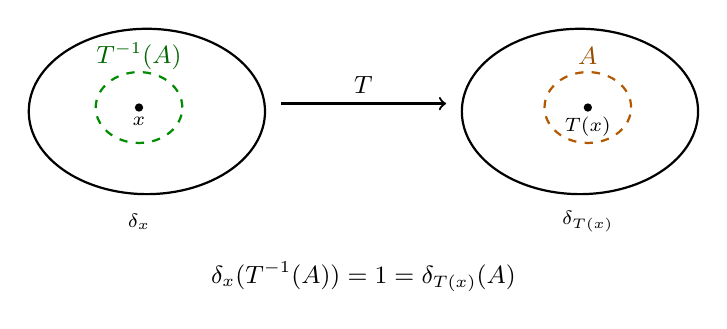
\begin{tikzpicture}[scale=1.0]
  % 左：X 側の楕円と点 x, 囲み T^{-1}(A)
  \draw[thick] (0, 0) ellipse (1.5cm and 1.05cm);
  \node[above right, font=\scriptsize, gray] at (-1.3, 0.7) {$\X$};
  \draw[dashed, thick, green!55!black]
    (-0.1, 0.05) ellipse (0.55cm and 0.45cm);
  \node[font=\small, green!40!black] at (-0.1, 0.7) {$T^{-1}(A)$};
  \fill (-0.1, 0.05) circle (1.5pt) node[below, font=\scriptsize] {$x$};

  % 矢印 T
  \draw[->, thick] (1.7, 0.1) -- (3.8, 0.1)
    node[midway, above, font=\small] {$T$};

  % 右：Y 側の楕円と点 T(x), 囲み A
  \begin{scope}[xshift=5.5cm]
    \draw[thick] (0, 0) ellipse (1.5cm and 1.05cm);
    \node[above right, font=\scriptsize, gray] at (-1.3, 0.7) {$\Y$};
    \draw[dashed, thick, orange!70!black]
      (0.1, 0.05) ellipse (0.55cm and 0.45cm);
    \node[font=\small, orange!60!black] at (0.1, 0.7) {$A$};
    \fill (0.1, 0.05) circle (1.5pt) node[below, font=\scriptsize] {$T(x)$};
  \end{scope}

  % 下：Dirac 測度の値
  \node[font=\scriptsize] at (-0.1, -1.4) {$\delta_x$};
  \node[font=\scriptsize] at (5.6, -1.4) {$\delta_{T(x)}$};
  \node[font=\small] at (2.75, -2.1)
    {$\delta_x(T^{-1}(A)) = 1 = \delta_{T(x)}(A)$};
\end{tikzpicture}
\end{center}

%% ============================================================
%% 凸解析
%% ============================================================
\section{凸解析}
\label{sec:sem-convex-analysis}

\subsection{凸結合と凸集合}
\label{sec:sem-convex}

\begin{definition}{凸集合（convex set）}{sem-convex}
  ベクトル空間 $V$ の部分集合 $S \subset V$ が\textbf{凸}であるとは，
  任意の $v_1, v_2 \in S$ と任意の $t \in [0,1]$ に対して
  \[
    t v_1 + (1-t) v_2 \in S
  \]
  が成り立つことをいう．
\end{definition}

\begin{definition}{凸多面体（convex polytope）}{sem-polytope}
  行列 $\mathbf{A} \in \R^{k \times d}$ とベクトル $\mathbf{b} \in \R^k$ に対して，
  線形等式・不等式制約で定まる $\R^d$ の部分集合
  \[
    \{\mathbf{x} \in \R^d \mid
      \mathbf{A}\mathbf{x} = \mathbf{b},\; \mathbf{x} \geq \mathbf{0}\}
  \]
  を\textbf{凸多面体}という．凸多面体は凸集合である．
\end{definition}
